\documentclass[xcolor=dvipsnames,table]{beamer}

\usepackage{latexsym}
\usepackage[utf8]{inputenc}
\usepackage[brazil]{babel}
\usepackage{amssymb}
\usepackage{amsmath}
\usepackage{stmaryrd}
\usepackage{fancybox}
\usepackage{datetime}
\usepackage[T1]{fontenc}
\usepackage{graphicx}
\usepackage{graphics}
\usepackage{url}
\usepackage{algorithmic}
\usepackage{algorithm}
\usepackage{acronym}
\usepackage{array}

\newtheorem{definicao}{Definio}
\newcommand{\tab}{\hspace*{2em}}

\mode<presentation>
{
  \definecolor{colortexto}{RGB}{0,0,0}
 
  \setbeamertemplate{background canvas}[vertical shading][ bottom=white!10,top=white!10]
  \setbeamercolor{normal text}{fg=colortexto} 

  \usetheme{Warsaw}
}

\title{Apresentação da disciplina} 

\author{
  Esdras Lins Bispo Jr. \\ \url{bispojr@ufg.br}
  } 
 \institute{
  Teoria de Grafos \\Bacharelado em Ciência da Computação}
\date{\textbf{02 de maio de 2017} }

\logo{
\includegraphics[width=1cm]{images/ufgJataiLogo.png}}

\begin{document}

	\begin{frame}
		\titlepage
	\end{frame}

	\AtBeginSection{
		\begin{frame}{Sumário}%[allowframebreaks]{Sumário}
    		\tableofcontents[currentsection]
    		%\tableofcontents[currentsection, hideothersubsections]
		\end{frame}
	}

	\begin{frame}{Plano de Aula}
		\tableofcontents
		%\tableofcontents[hideallsubsections]
	\end{frame}
	
	\section{Sobre a Disciplina}
	\subsection{Professor}
	\begin{frame}{Professor}
		\begin{columns}
			\column{.4\textwidth}  		
			\begin{center}
				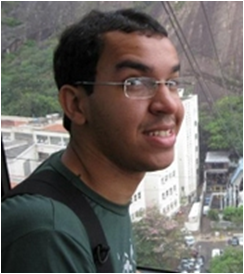
\includegraphics[height=.5\textheight]{images/esdras.png}
			\end{center}
			\column{.6 \textwidth}  		
			\begin{block}{Formação}
				\begin{center}
					{\normalsize {\bf Bacharel} em Sistemas de Informação\\
						{\bf Mestre} em Representação Conhecimento (IA)}
				\end{center}
			\end{block}		  		
			\begin{block}{Quem?}
				\begin{center}
					{\bf Esdras Lins Bispo Junior} \\ Recife, Pernambuco.
				\end{center}
			\end{block}
		\end{columns}
	\end{frame}
	
	\subsection{Informações Importantes}
	\begin{frame}{Informações Importantes}
		\begin{block}{Professor}
			\begin{itemize}
				\item Esdras Lins Bispo Jr.
				\item \url{bispojr@ufg.br}
				\item Sala 18, 1º Andar (Bloco Novo dos Professores)
			\end{itemize}
		\end{block}
	\end{frame}	
	
	\begin{frame}{Informações Importantes}
		\begin{block}{Disciplina}
			\begin{itemize}
				\item Teoria de Grafos
				\item 15h30-17h10 (Terça, CA 1, Sala 12)\\
				09h30-11h10 (Quarta, CA 1, Sala 14)
				\item Dúvidas: 17h30 - 19h00 (Quinta)\\
				{\color{red}[é necessário confirmação comigo]}
				\item \url{www.facebook.com/groups/tg.rej.2017.1/}
			\end{itemize}
		\end{block}
	\end{frame}
	
	\begin{frame}{Informações Importantes}
		\begin{block}{Metodologia}
			\begin{itemize}
				\item Ensino sob Medida (Novak, 2011);
				\item Aulas expositivas utilizando quadro negro (ou branco) e DataShow;
				\item Atendimento individual ou em grupos;
				\item Aplicação de listas de exercícios;
				\item Aplicação de atividades de aquecimento utilizando o 
				Canvas AVA (Ambiente Virtual de Aprendizagem);
				\item Tempo de Aula: 50 minutos.
			\end{itemize}
		\end{block}
	\end{frame}
	
	\subsection{Instrumentos de Avaliação}
	\begin{frame}{Instrumentos de Avaliação}
		\begin{block}{Mini-Testes (Previsão de datas)}
			\begin{itemize}
				\item MT$_1$ $\Rightarrow$ 20\% da pontuação total (16 de maio);
				\item MT$_2$ $\Rightarrow$ 20\% da pontuação total (07 de junho);
				\item MT$_3$ $\Rightarrow$ 20\% da pontuação total (28 de junho);
				\item MT$_4$ $\Rightarrow$  20\% da pontuação total (16 de agosto).
			\end{itemize}
		\end{block} \pause
		\begin{block}{Exercício de Aquecimento (EA)}
			Serão propostos EAs, durante toda a disciplina, equivalendo a 10\% da pontuação total.
		\end{block}
	\end{frame}
	
	\begin{frame}{Instrumentos de Avaliação}
		\begin{block}{Prova Final (PF) - 20\% da pontuação total}
			A PF é composta por duas etapas: \pause
			\begin{itemize}
				\item a PF$_1$ (29 de agosto) e
				\item a PF$_2$ (06 de setembro).
			\end{itemize}  \pause
			A PF$_1$ é composta por dois mini-testes de caráter substitutivo: \pause 
			\begin{itemize}
				\item o SMT$_1$ (referente ao MT$_1$), e 
				\item o SMT$_2$ (referente ao MT$_2$).
			\end{itemize} \pause
			Por sua vez, a PF$_2$ é composta pelos outros dois mini-testes também de caráter substitutivo:  \pause
			\begin{itemize}
				\item o SMT$_3$ (referente ao MT$_3$), e 
				\item o SMT$_4$ (referente ao MT$_4$).
			\end{itemize}
		\end{block}
	\end{frame}
	
	\begin{frame}{Avaliação}
		\begin{block}{Média Final}
			O cálculo da média final será dada da seguinte forma:
			\begin{itemize}
				\item MF = MIN(10, PONT)
			\end{itemize}
			em que MIN representa o mínimo entre dois valores e PONT representa a pontuação total obtida em toda a disciplina, dada da seguinte forma:
			\begin{center}
				PONT = $\left[ \sum\limits_{i=1}^{4} \mbox{max}(MT_i, SMT_i) + PF \right] \times 0,2 + EA \times 0,1$
			\end{center}
		\end{block} \pause
		\begin{exampleblock}{Previsão de Término das Atividades}
			06 de setembro de 2017
		\end{exampleblock}
	\end{frame}
	
	\subsection{Distintivos Digitais}
	\begin{frame}{Distintivos Digitais}
		\begin{block}{Como será?}
			Os alunos que estiverem entre as 10 melhores notas de cada avaliação receberão um distintivo digital.
		\end{block} \pause
		\begin{block}{Quantos distintivos existem?}
			\begin{itemize}
				\item {\sc Top One}
				\item {\sc Top Five}
				\item {\sc Top Ten}
			\end{itemize}
		\end{block}
	\end{frame}
	
	\begin{frame}{Distintivos Digitais}
		\begin{block}{}
			\begin{center}
				
\includegraphics[height=.65\textheight]{images/badges/top-ten.png}
			\end{center}		
			Obter a 6ª ou até a 10ª melhor nota da turma em uma avaliação. 
		\end{block}
	\end{frame}
	
	\begin{frame}{Distintivos Digitais}
		\begin{block}{}
			\begin{center}
				
\includegraphics[height=.65\textheight]{images/badges/top-five.png}
			\end{center}		
			Obter a 2ª ou até a 5ª melhor nota da turma em uma avaliação. 
		\end{block}
	\end{frame}
	
	\begin{frame}{Distintivos Digitais}
		\begin{block}{}
			\begin{center}
				
\includegraphics[height=.65\textheight]{images/badges/top-one.png}
			\end{center}		
			Obter a melhor nota da turma em uma avaliação. 
		\end{block}
	\end{frame}
	
	\begin{frame}{Distintivos Digitais}
		\begin{block}{Pontuação}
			\begin{itemize}
				\item Obter um {\sc Top One}: 12 pontos;
				\item Obter um {\sc Top Five}: 6 pontos;
				\item Obter um {\sc Top Ten}: 3 pontos.
			\end{itemize}
		\end{block} \pause
		\begin{block}{Por que estamos usando distintivos digitais?}
			\begin{itemize}
				\item Pode aumentar a motivação dos alunos; \\ \pause
				{\color{blue} (Estou pesquisando para saber se isto é verdade...)}
			\end{itemize}
		\end{block}
	\end{frame}

	\begin{frame}{Distintivos Digitais}
		\begin{exampleblock}{No final da disciplina...}
			Os dez primeiros que obtiverem maior pontuação ganharão medalhas.
		\end{exampleblock} \pause
		\begin{center}
			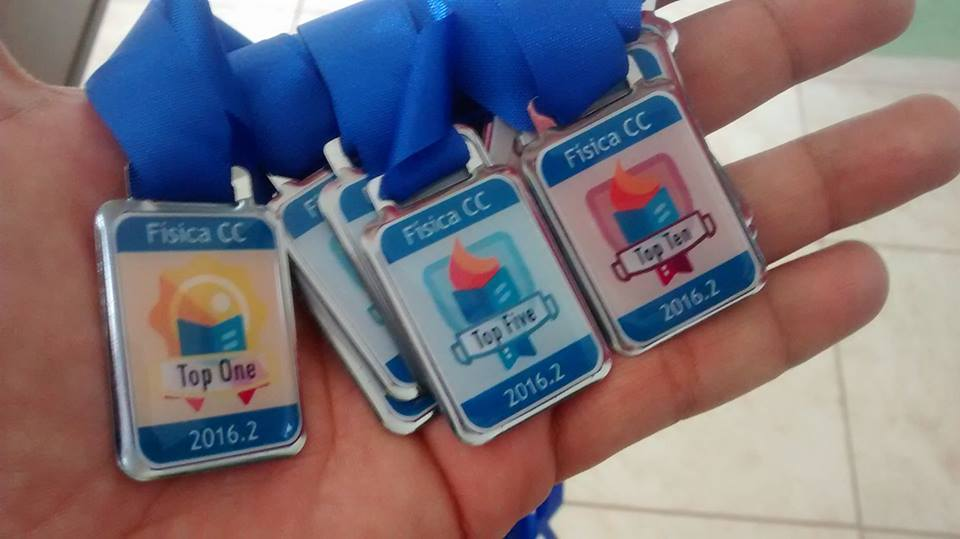
\includegraphics[height=.6\textheight]{images/badges/medalhas}
		\end{center}
	\end{frame}

	\begin{frame}{Informações Importantes}
		\begin{block}{Conteúdo do Curso}
			\begin{enumerate}
				\item Noções Básicas de Grafos;
				\item Circuitos e Caminhos;
				\item Subgrafos;
				\item Grafos Conexos e Componentes;
				\item Cortes e Pontes;
			\end{enumerate}
		\end{block}
	\end{frame}
	
	\begin{frame}{Informações Importantes}
		\begin{block}{Conteúdo do Curso}
			\begin{enumerate}
				\item Árvores;
				\item Isomorfismo;
				\item Coloração;
				\item Planaridade;				
				\item Outros Tópicos.
			\end{enumerate}
		\end{block}
	\end{frame}

%------------------------------------------
	\section{Pensamento}
	\begin{frame}{Pensamento}
  		\begin{center}
    		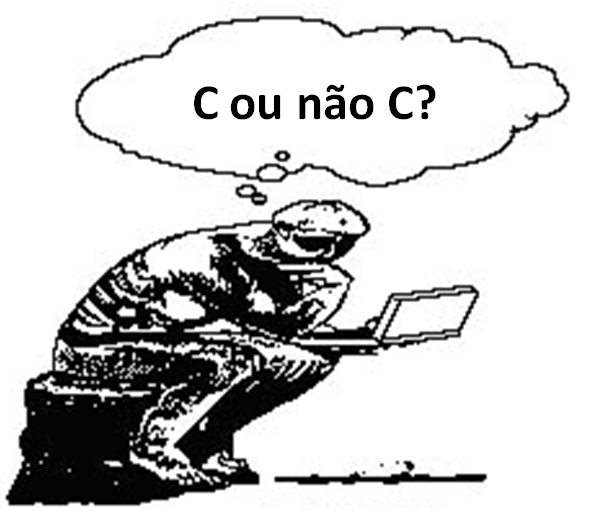
\includegraphics[width=7cm]{images/pensamento.png}
  		\end{center}
	\end{frame}
	
	\begin{frame}{Pensamento}
		\begin{columns}
			\column{.4\textwidth}  		
		  		\begin{center}
		    		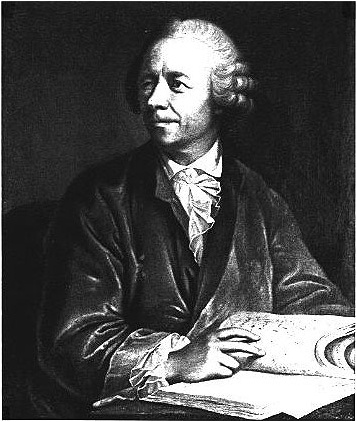
\includegraphics[height=.5\textheight]{images/euler.png}
		  		\end{center}
			\column{.6\textwidth}  		
				\begin{block}{Frase}
					\begin{center}
						{\large Now I will have less distraction.}
					\end{center}
				\end{block}		  		
		  		\begin{block}{Quem?}
		  			\begin{center}
						{\bf Leonhard Euler (1707-83)} \\ Matemático e físico suíço.
					\end{center}
				\end{block}
		\end{columns}
	\end{frame}
%------------------------------------------
	\section{Problemas em Grafos}
	\subsection{O problema de Euler}
	\begin{frame}[shrink]{O problema de Euler}
		\begin{center}
    		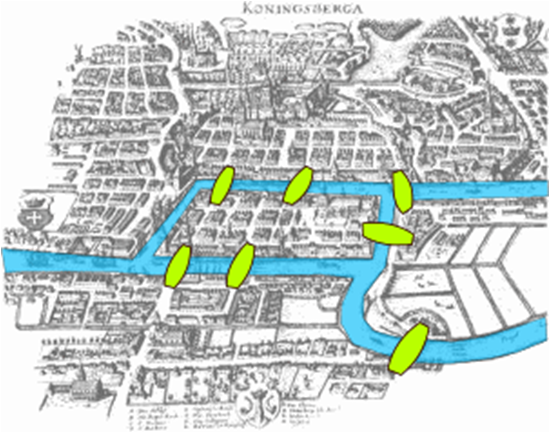
\includegraphics[height=.6\textheight]{images/konigsberg.png}
  		\end{center} \pause
		\begin{alertblock}{Sete pontes de Konigsberg} \pause
			É possível cruzar as setes pontes sem passar \\
			duas vezes por nenhuma delas?
		\end{alertblock}
	\end{frame}
	
	\begin{frame}[shrink]{O problema de Euler}
		\begin{center}
    		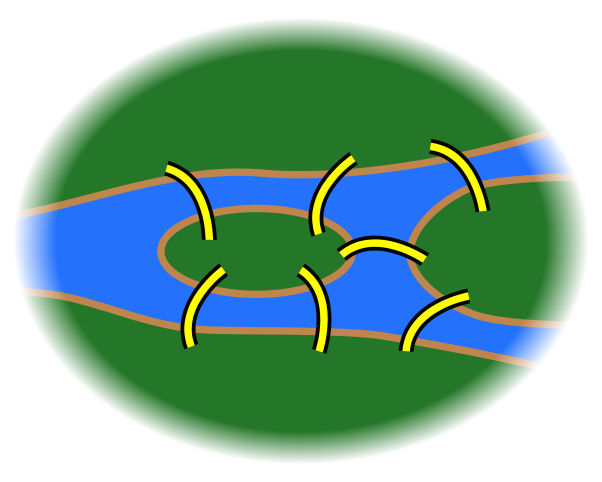
\includegraphics[height=.6\textheight]{images/konigsberg2.png}
  		\end{center} 
		\begin{alertblock}{Sete pontes de Konigsberg} 
			É possível cruzar as setes pontes sem passar \\
			duas vezes por nenhuma delas?
		\end{alertblock}
	\end{frame}
	
	\begin{frame}{O problema de Euler}
		\begin{center}
    		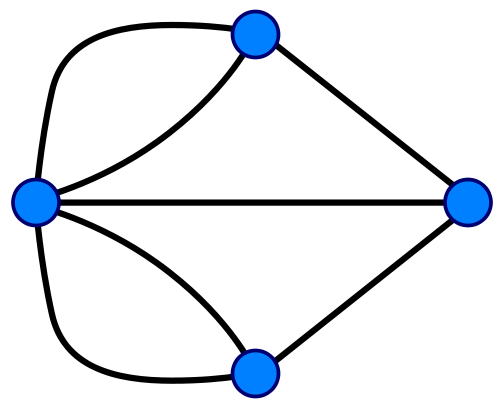
\includegraphics[height=.6\textheight]{images/konigsberg3.png}
  		\end{center} 
		\begin{block}{Sete pontes de Konigsberg} \pause
			Apresentado em 1736.
		\end{block}
	\end{frame}
	
	\subsection{O problema de Guthrie}
	\begin{frame}[shrink]{O problema de Guthrie}
		\begin{center}
    		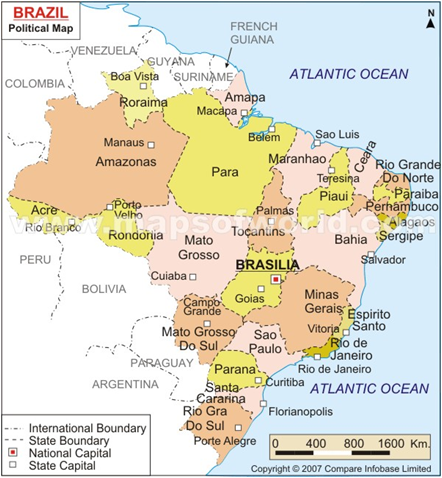
\includegraphics[height=.6\textheight]{images/mapa.png}
  		\end{center} \pause
		\begin{alertblock}{Coloração de Mapas} \pause
			É verdade que quatro cores são suficientes \\
			para se colorar um mapa plano?
		\end{alertblock}
	\end{frame}
	
	\begin{frame}[shrink]{O problema de Guthrie}
		\begin{center}
    		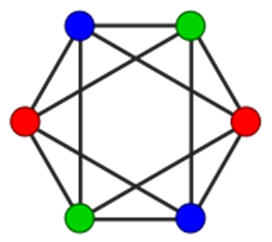
\includegraphics[height=.6\textheight]{images/grafoColorido.png}
  		\end{center}
		\begin{alertblock}{Coloração de Mapas}
			É verdade que quatro cores são suficientes \\
			para se colorar um mapa plano?
		\end{alertblock}
	\end{frame}
	
	\begin{frame}{O problema de Guthrie}
		\begin{center}
    		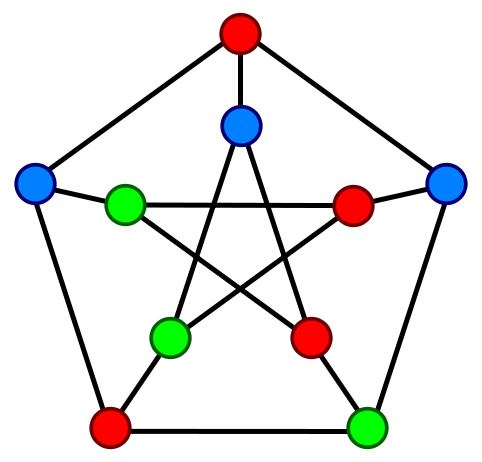
\includegraphics[height=.6\textheight]{images/grafoColorido2.png}
  		\end{center}
		\begin{block}{Coloração de Mapas} \pause
			Apresentado em 1852. Provado em 1976.
		\end{block}
	\end{frame}
	
	\subsection{O problema do menor caminho}
	\begin{frame}{O problema do menor caminho}
		\begin{center}
    		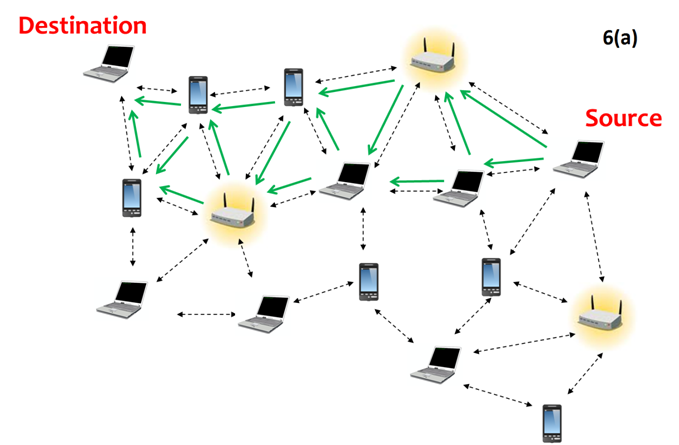
\includegraphics[height=.6\textheight]{images/redes.png}
  		\end{center}
		\begin{alertblock}{Menor Caminho} \pause
			Qual é o roteamento de menor custo entre dois dispositivos?
		\end{alertblock}
	\end{frame}
	
	\begin{frame}{O problema do menor caminho}
		\begin{center}
    		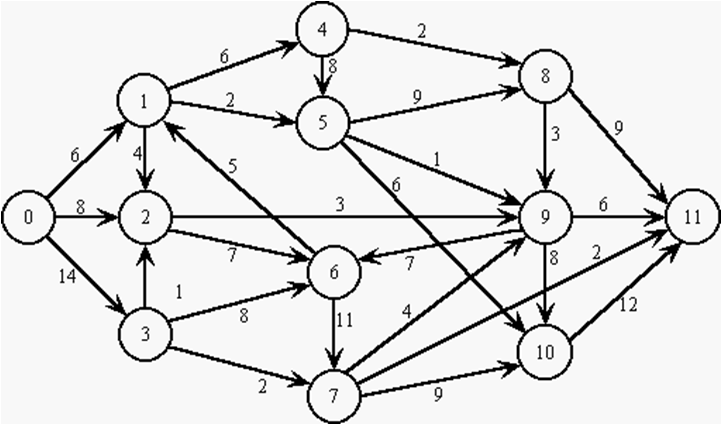
\includegraphics[height=.6\textheight]{images/redesGrafo.png}
  		\end{center}
		\begin{block}{Menor Caminho} \pause
			Algoritmo de Dijkstra (proposto em 1959).
		\end{block}
	\end{frame}
	
	\begin{frame}{O que existe em comum nos três problemas?} \pause
		\begin{block}{Modelo} \pause
			Um modelo é uma {\bf simplificação} da realidade. Um modelo abstrai algumas informações e se concentra em outras informações.
		\end{block} \pause
		\begin{block}{Bom modelo}
			Um bom modelo é aquele que consegue descrever com maior proximidade as características essenciais do problema.
		\end{block}
	\end{frame}
	
	\section{Noções Básicas de Grafos}	
	\begin{frame}{Noções Básicas de Grafos}
		\begin{block}{$V^{(2)}$}
			Para qualquer conjunto $V$, denotaremos por $V^{(2)}$ o conjunto de todos os pares não-ordenados de elementos distintos de $V$.
		\end{block}
	\end{frame}
	
	\begin{frame}
		\titlepage
	\end{frame}
	
\end{document}